%----PrefaceImport----%
\documentclass{article}
\usepackage{fancyhdr}
\usepackage[a4paper,margin=1in,headsep=25pt]{geometry}
\usepackage{lipsum,hyperref}
\usepackage{enumerate,fullpage,proof}
\usepackage[fontsize=12pt]{fontsize}
\usepackage{amsmath,amscd,amsbsy,amssymb,latexsym,url,bm,amsthm}
\usepackage{epsfig,graphicx,subfigure}
\usepackage{listings}
\usepackage{bbm}
\usepackage[usenames]{xcolor}

\newtheorem{thm}{Theorem}
\newtheorem{lemma}[thm]{Lemma}

\pagestyle{fancy}
\pagenumbering{Alph}
\setlength{\headheight}{36.0pt}
\headsep = 25pt
\fancyhf{}
\lhead{CSE 4392 Special Topic: Natural Language Processing}
\rhead{Homework 9: Recurrent Neural Networks}
\lfoot{2024 Kenny Zhu}
%----Documentation----%
\begin{document}

\title{CSE 4392 Special Topic: Natural Language Processing}
\author{Homework 9 - Spring 2024}
\date{Due Date: Apr 9th, 2024, 11:59 p.m. Central Standard Time}
\maketitle
\thispagestyle{fancy}

%----Homeworks----%

This week, we explored Recurrent Neural Networks (RNNs) and their variations, focusing on their implementation in Natural Language Processing (NLP). We covered the fundamentals of RNNs and their limitations like the vanishing gradient problem, and introduced Long Short-Term Memory (LSTM) networks as a solution. Moreover, we discussed Bidirectional RNNs (BiRNNs), which process input sequences in both forward and backward directions to capture context from past and future inputs. Finally, we applied these concepts to understand how RNNs, LSTMs, and BiRNNs can be effectively utilized in various tasks.
\section*{Problem 1 - 100\%}

This week's homework delves into the realm of Recurrent Neural Networks (RNNs) and their variants, focusing on their application in text classification tasks(MBTI Classification). The assignment comprises two questions aimed at reinforcing your understanding of RNNs and Bi-directional RNNs (BiRNNs) for text classification:

\subsection*{Question 1 - 40\%}
In this question, you'll undertake the mathematical derivation of the gradients for parameters within a Bi-directional RNN model tailored for text classification. Your task involves computing gradients with respect to the model's parameters, including input-to-hidden weights, hidden-to-hidden weights, and biases.

Recall we learned the derivation of the gradients for RNNs as:
$$\frac{\partial L }{\partial \mathbf{W}} = -\frac{1}{n}\sum_{t=1}^{n}\sum_{k=1}^{t}  \frac{\partial L_t }{\partial  \mathbf{h}_t}\left ( \prod_{j=k+1}^{t}  \frac{\partial \mathbf{h}_j  }{\partial  \mathbf{h}_{j-1}} \right ) \frac{\partial \mathbf{h}_k }{\partial \mathbf{W}},$$
If we follow the implementation of BiRNNs as below:
\begin{align}
    f_1(\mathbf{h}, \mathbf{x}) &= g(\mathbf{W}_1\mathbf{h} + \mathbf{U}_1\mathbf{x} + b_1)\\
    f_2(\mathbf{h}, \mathbf{x}) &= g(\mathbf{W}_2\mathbf{h} + \mathbf{U}_2\mathbf{x} + b_2)\\
    \overrightarrow{\mathbf{h}}_t &= f_1(\overrightarrow{\mathbf{h}}_{t-1}, \mathbf{x}_t), t=1,2,...,n\\
    \overleftarrow{\mathbf{h}}_t &=  f_2(\overrightarrow{\mathbf{h}}_{t-1}, \mathbf{x}_t), t=n,n-1,...,1\\
    \mathbf{h}_t &= \left [ \overrightarrow{\mathbf{h}_t}, \overleftarrow{\mathbf{h}_t} \right ] \in \mathbb{R}^{2d}\\
    P(y_i=k) &= softmax_k(\mathbf{W}_o \mathbf{h}_t)\\
   L &= -\frac{1}{n}\sum_{n}^{i=1}\log P(y_i=k)  
   \end{align}
Please derive the gradients for parameters $\mathbf{W}_0$, $\mathbf{W}_1$, $\mathbf{W}_2$, $\mathbf{U}_1$, $\mathbf{U}_2$, $\mathbf{b}_1$, $\mathbf{b}_2$, in a Bi-directional RNN model.

\subsection*{Question 2 - 60\%}

Hope your final project is going well!
For implementing your final project,
you must have a taste of deep learning platforms like PyTorch.

In this question, you are tasked with implementing a bidirectional 
Long Short-Term Memory (LSTM) model
for text classification using PyTorch. 

Although we just learned the Bi-directional RNNs in class,
you can easily implement a Bi-directional LSTM model in PyTorch.
The architecture of the BiLSTM model is shown as below:

\begin{figure}[h]
    \centering
    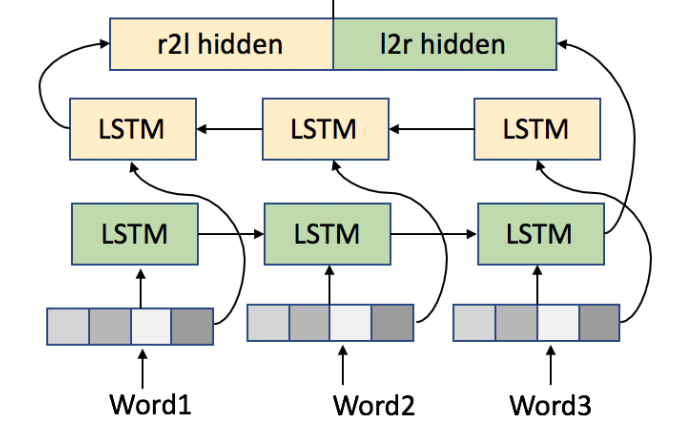
\includegraphics[width=0.6\textwidth]{bi-dir-lstm.png}
    \caption{Bidirectional LSTM Model Architecture}
\end{figure}

However, \textbf{you are not allowed to use PyTorch's built-in bidirectional LSTM module},
which means you \textcolor{red}{cannot} use the \texttt{torch.nn.LSTM} module with the \texttt{bidirectional=True} flag. 
Instead, you will manually implement the bidirectional functionality 
by concatenating the outputs of two separate LSTM layers: 
one processing the input sequence in the forward direction and 
the other in the backward direction.

\subsection*{Description:}
\begin{enumerate}
    \item \textbf{Define the Model Architecture:} Implement the \texttt{BiLSTM} function, which takes input parameters such as \texttt{input\_size}, \texttt{hidden\_size}, \texttt{num\_layers}, and \texttt{output\_size}. Inside this function, define two separate LSTM layers (\texttt{lstm\_forward} and \texttt{lstm\_backward}) to process the input sequence in forward and backward directions, respectively.
    
    \item \textbf{Forward Pass:} Define the forward pass function inside the \texttt{BiLSTM} function. Initialize the hidden and cell states for both forward and backward LSTMs, perform the forward pass with the forward LSTM, reverse the input sequence, perform the forward pass with the backward LSTM, and concatenate the outputs of both LSTMs along the feature dimension.
    
    \item \textbf{Output Layer:} Add a linear layer (\texttt{fc}) to transform the concatenated output of the bidirectional LSTMs to the desired output size (number of classes for classification).
    
    \item \textbf{Training Loop:} Instantiate the \texttt{BiLSTM} model with appropriate parameters. Define the loss function (e.g., CrossEntropyLoss) and optimizer (e.g., Adam). Train the model on the provided dataset using a suitable training loop, optimizing the model parameters to minimize the loss.
    
    \item \textbf{Evaluation:} After training, evaluate the model's performance on a separate validation or test dataset. Calculate relevant evaluation metrics such as accuracy, precision, recall, and F1-score to assess the model's classification performance.
\end{enumerate}

\textbf{Attach your codes and report.}

\end{document}



